%%%%%%%%%%%%%%%%%%%%%%%%%%%%%%%%%%%%%%%%%%%%%%%%%%%%%%%%%%%%%%%%%%%%%%%%%%
%
% 	Template for seminar reports
%
%%%%%%%%%%%%%%%%%%%%%%%%%%%%%%%%%%%%%%%%%%%%%%%%%%%%%%%%%%%%%%%%%%%%%%%%%%

%%%%%%%%%%%%%%%%%%%%%%%%%%%%%%%%%%%%%%%%%%%%%%%%%%%%%%%%%%%%%%%%%%%%%%%%%%
% 	Include layout and macros
%%%%%%%%%%%%%%%%%%%%%%%%%%%%%%%%%%%%%%%%%%%%%%%%%%%%%%%%%%%%%%%%%%%%%%%%%%



%% This LaTeX template is based on the following example file included in the ieeetran
%% package:
%% bare_conf.tex 
%% V1.2
%% 2002/11/18
%% by Michael Shell
%% mshell@ece.gatech.edu
%% (requires IEEEtran.cls version 1.6b or later) with an IEEE conference paper.


% Note that the a4paper option is mainly intended so that authors in
% countries using A4 can easily print to A4 and see how their papers will
% look in print. Authors are encouraged to use U.S. letter paper when 
% submitting to IEEE. Use the testflow package mentioned above to verify
% correct handling of both paper sizes by the author's LaTeX system.
%
% Also note that the "draftcls" or "draftclsnofoot", not "draft", option
% should be used if it is desired that the figures are to be displayed in
% draft mode.
%
% This paper can be formatted using the peerreviewca
% (instead of conference) mode.
\documentclass[conference, a4paper]{IEEEtran-modified}
% If the IEEEtran.cls has not been installed into the LaTeX system files, 
% manually specify the path to it:
% \documentclass[conference]{../sty/IEEEtran} 

\IEEEoverridecommandlockouts{}

% some very useful LaTeX packages include:

\usepackage{cite}       % Written by Donald Arseneau
                        % V1.6 and later of IEEEtran pre-defines the format
                        % of the cite.sty package \cite{} output to follow
                        % that of IEEE. Loading the cite package will
                        % result in citation numbers being automatically
                        % sorted and properly "ranged". i.e.,
                        % [1], [9], [2], [7], [5], [6]
                        % (without using cite.sty)
                        % will become:
                        % [1], [2], [5]--[7], [9] (using cite.sty)
                        % cite.sty's \cite will automatically add leading
                        % space, if needed. Use cite.sty's noadjust option
                        % (cite.sty V3.8 and later) if you want to turn this
                        % off. cite.sty is already installed on most LaTeX
                        % systems. The latest version can be obtained at:
                        % http://www.ctan.org/tex-archive/macros/latex/contrib/supported/cite/

%\usepackage{graphicx}  % Written by David Carlisle and Sebastian Rahtz
                        % Required if you want graphics, photos, etc.
                        % graphicx.sty is already installed on most LaTeX
                        % systems. The latest version and documentation can
                        % be obtained at:
                        % http://www.ctan.org/tex-archive/macros/latex/required/graphics/
                        % Another good source of documentation is "Using
                        % Imported Graphics in LaTeX2e" by Keith Reckdahl
                        % which can be found as esplatex.ps and epslatex.pdf
                        % at: http://www.ctan.org/tex-archive/info/
% NOTE: for dual use with latex and pdflatex, instead load graphicx like:
\ifx\pdfoutput\undefined{}
	\usepackage{graphicx}
\else
	\usepackage[pdftex]{graphicx}
\fi

% However, be warned that pdflatex will require graphics to be in PDF
% (not EPS) format and will preclude the use of PostScript based LaTeX
% packages such as psfrag.sty and pstricks.sty. IEEE conferences typically
% allow PDF graphics (and hence pdfLaTeX). However, IEEE journals do not
% (yet) allow image formats other than EPS or TIFF. Therefore, authors of
% journal papers should use traditional LaTeX with EPS graphics.
%
% The path(s) to the graphics files can also be declared: e.g.,
% \graphicspath{{../eps/}{../ps/}}
% if the graphics files are not located in the same directory as the
% .tex file. This can be done in each branch of the conditional above
% (after graphicx is loaded) to handle the EPS and PDF cases separately.
% In this way, full path information will not have to be specified in
% each \includegraphics command.
%
% Note that, when switching from latex to pdflatex and vice-versa, the new
% compiler will have to be run twice to clear some warnings.
\graphicspath{{figures/}}


%\usepackage{psfrag}    % Written by Craig Barratt, Michael C. Grant,
                        % and David Carlisle
                        % This package allows you to substitute LaTeX
                        % commands for text in imported EPS graphic files.
                        % In this way, LaTeX symbols can be placed into
                        % graphics that have been generated by other
                        % applications. You must use latex->dvips->ps2pdf
                        % workflow (not direct pdf output from pdflatex) if
                        % you wish to use this capability because it works
                        % via some PostScript tricks. Alternatively, the
                        % graphics could be processed as separate files via
                        % psfrag and dvips, then converted to PDF for
                        % inclusion in the main file which uses pdflatex.
                        % Docs are in "The PSfrag System" by Michael C. Grant
                        % and David Carlisle. There is also some information 
                        % about using psfrag in "Using Imported Graphics in
                        % LaTeX2e" by Keith Reckdahl which documents the
                        % graphicx package (see above). The psfrag package
                        % and documentation can be obtained at:
                        % http://www.ctan.org/tex-archive/macros/latex/contrib/supported/psfrag/

%\usepackage{subfigure} % Written by Steven Douglas Cochran
                        % This package makes it easy to put subfigures
                        % in your figures. i.e., "figure 1a and 1b"
                        % Docs are in "Using Imported Graphics in LaTeX2e"
                        % by Keith Reckdahl which also documents the graphicx
                        % package (see above). subfigure.sty is already
                        % installed on most LaTeX systems. The latest version
                        % and documentation can be obtained at:
                        % http://www.ctan.org/tex-archive/macros/latex/contrib/supported/subfigure/

%\usepackage{url}       % Written by Donald Arseneau
                        % Provides better support for handling and breaking
                        % URLs. url.sty is already installed on most LaTeX
                        % systems. The latest version can be obtained at:
                        % http://www.ctan.org/tex-archive/macros/latex/contrib/other/misc/
                        % Read the url.sty source comments for usage information.

%\usepackage{stfloats}  % Written by Sigitas Tolusis
                        % Gives LaTeX2e the ability to do double column
                        % floats at the bottom of the page as well as the top.
                        % (e.g., "\begin{figure*}[!b]" is not normally
                        % possible in LaTeX2e). This is an invasive package
                        % which rewrites many portions of the LaTeX2e output
                        % routines. It may not work with other packages that
                        % modify the LaTeX2e output routine and/or with other
                        % versions of LaTeX. The latest version and
                        % documentation can be obtained at:
                        % http://www.ctan.org/tex-archive/macros/latex/contrib/supported/sttools/
                        % Documentation is contained in the stfloats.sty
                        % comments as well as in the presfull.pdf file.
                        % Do not use the stfloats baselinefloat ability as
                        % IEEE does not allow \baselineskip to stretch.
                        % Authors submitting work to the IEEE should note
                        % that IEEE rarely uses double column equations and
                        % that authors should try to avoid such use.
                        % Do not be tempted to use the cuted.sty or
                        % midfloat.sty package (by the same author) as IEEE
                        % does not format its papers in such ways.

\usepackage{amsmath}    % From the American Mathematical Society
                        % A popular package that provides many helpful commands
                        % for dealing with mathematics. Note that the AMSmath
                        % package sets \interdisplaylinepenalty to 10000 thus
                        % preventing page breaks from occurring within multiline
                        % equations. Use:
\interdisplaylinepenalty=2500
                        % after loading amsmath to restore such page breaks
                        % as IEEEtran.cls normally does. amsmath.sty is already
                        % installed on most LaTeX systems. The latest version
                        % and documentation can be obtained at:
                        % http://www.ctan.org/tex-archive/macros/latex/required/amslatex/math/



% Other popular packages for formatting tables and equations include:

%\usepackage{array}
% Frank Mittelbach's and David Carlisle's array.sty which improves the
% LaTeX2e array and tabular environments to provide better appearances and
% additional user controls. array.sty is already installed on most systems.
% The latest version and documentation can be obtained at:
% http://www.ctan.org/tex-archive/macros/latex/required/tools/

% Mark Wooding's extremely powerful MDW tools, especially mdwmath.sty and
% mdwtab.sty which are used to format equations and tables, respectively.
% The MDWtools set is already installed on most LaTeX systems. The lastest
% version and documentation is available at:
% http://www.ctan.org/tex-archive/macros/latex/contrib/supported/mdwtools/


% V1.6 of IEEEtran contains the IEEEeqnarray family of commands that can
% be used to generate multiline equations as well as matrices, tables, etc.


% Also of notable interest:

% Scott Pakin's eqparbox package for creating (automatically sized) equal
% width boxes. Available:
% http://www.ctan.org/tex-archive/macros/latex/contrib/supported/eqparbox/



% Notes on hyperref:
% IEEEtran.cls attempts to be compliant with the hyperref package, written
% by Heiko Oberdiek and Sebastian Rahtz, which provides hyperlinks within
% a document as well as an index for PDF files (produced via pdflatex).
% However, it is a tad difficult to properly interface LaTeX classes and
% packages with this (necessarily) complex and invasive package. It is
% recommended that hyperref not be used for work that is to be submitted
% to the IEEE. Users who wish to use hyperref *must* ensure that their
% hyperref version is 6.72u or later *and* IEEEtran.cls is version 1.6b 
% or later. The latest version of hyperref can be obtained at:
%
% http://www.ctan.org/tex-archive/macros/latex/contrib/supported/hyperref/
%
% Also, be aware that cite.sty (as of version 3.9, 11/2001) and hyperref.sty
% (as of version 6.72t, 2002/07/25) do not work optimally together.
% To mediate the differences between these two packages, IEEEtran.cls, as
% of v1.6b, predefines a command that fools hyperref into thinking that
% the natbib package is being used - causing it not to modify the existing
% citation commands, and allowing cite.sty to operate as normal. However,
% as a result, citation numbers will not be hyperlinked. Another side effect
% of this approach is that the natbib.sty package will not properly load
% under IEEEtran.cls. However, current versions of natbib are not capable
% of compressing and sorting citation numbers in IEEE's style - so this
% should not be an issue. If, for some strange reason, the user wants to
% load natbib.sty under IEEEtran.cls, the following code must be placed
% before natbib.sty can be loaded:
%
% \makeatletter
% \let\NAT@parse\undefined
% \makeatother
%
% Hyperref should be loaded differently depending on whether pdflatex
% or traditional latex is being used:
%
%\ifx\pdfoutput\undefined
%\usepackage[hypertex]{hyperref}
%\else
%\usepackage[pdftex,hypertexnames=false]{hyperref}
%\fi
%
% Pdflatex produces superior hyperref results and is the recommended
% compiler for such use.



% *** Do not adjust lengths that control margins, column widths, etc. ***
% *** Do not use packages that alter fonts (such as pslatex).         ***
% There should be no need to do such things with IEEEtran.cls V1.6 and later.

%%%%%%%%%%%%%%%%%%%%%%%%%%%%%%%%%%%%%%%%%%%%%%%%%%%%%%%%%%%%%%%%%%%%%%%%%%
% 	Anpassung an deutsche Texte
%%%%%%%%%%%%%%%%%%%%%%%%%%%%%%%%%%%%%%%%%%%%%%%%%%%%%%%%%%%%%%%%%%%%%%%%%%

%\usepackage{ngerman}
\usepackage[utf8]{inputenc}  
\usepackage{tikz, pgfplots}
\usepackage{amsfonts}
\pgfplotsset{compat=1.18}
\usepackage{pgfplots}
\DeclareUnicodeCharacter{2212}{−}
\usepgfplotslibrary{groupplots,dateplot}
\usetikzlibrary{patterns,shapes.arrows}
\pgfplotsset{compat=newest}
\usepackage{booktabs}
\usepackage{url}
\usepackage{xurl}
\usepackage{subcaption}
\usepackage[hidelinks]{hyperref}
\usepackage{cleveref}
\usepackage{flushend}


%%%%%%%%%%%%%%%%%%%%%%%%%%%%%%%%%%%%%%%%%%%%%%%%%%%%%%%%%%%%%%%%%%%%%%%%%%
% 	Page numbering (not on first page)
%%%%%%%%%%%%%%%%%%%%%%%%%%%%%%%%%%%%%%%%%%%%%%%%%%%%%%%%%%%%%%%%%%%%%%%%%%
\pagestyle{empty}

%%%%%%%%%%%%%%%%%%%%%%%%%%%%%%%%%%%%%%%%%%%%%%%%%%%%%%%%%%%%%%%%%%%%%%%%%%
% 	Correct bad hyphenation here
%%%%%%%%%%%%%%%%%%%%%%%%%%%%%%%%%%%%%%%%%%%%%%%%%%%%%%%%%%%%%%%%%%%%%%%%%%

\hyphenation{}

%%%%%%%%%%%%%%%%%%%%%%%%%%%%%%%%%%%%%%%%%%%%%%%%%%%%%%%%%%%%%%%%%%%%%%%%%%
% 	Begin of the document
%%%%%%%%%%%%%%%%%%%%%%%%%%%%%%%%%%%%%%%%%%%%%%%%%%%%%%%%%%%%%%%%%%%%%%%%%%

\setlength{\marginparwidth}{5cm}
%\usepackage{todonotes}
%\newcommand{\todok}[1]{\todo[color=red!50, linecolor=black!50!red, inline]{#1}}


\begin{document}

%%%%%%%%%%%%%%%%%%%%%%%%%%%%%%%%%%%%%%%%%%%%%%%%%%%%%%%%%%%%%%%%%%%%%%%%%%
% 	Paper title
%%%%%%%%%%%%%%%%%%%%%%%%%%%%%%%%%%%%%%%%%%%%%%%%%%%%%%%%%%%%%%%%%%%%%%%%%%

\title{ Adaptive Sparse Grids}

%%%%%%%%%%%%%%%%%%%%%%%%%%%%%%%%%%%%%%%%%%%%%%%%%%%%%%%%%%%%%%%%%%%%%%%%%%
% 	Author names and affiliations 
%		-	multiple columns for up to three different affilitations are separated 
%			by \and
%		- for over three affiliations, refer to ieeetran howto
%%%%%%%%%%%%%%%%%%%%%%%%%%%%%%%%%%%%%%%%%%%%%%%%%%%%%%%%%%%%%%%%%%%%%%%%%%

\author{
    \authorblockN{Muhammed Kürşat Yurt}
    \authorblockA{TUM School of Computation, Information and Technology\\
        Technische Universität München
        Email: kursat.yurt@tum.de}
    %\and
    %\authorblockN{}
    %\authorblockA{}
}

%%%%%%%%%%%%%%%%%%%%%%%%%%%%%%%%%%%%%%%%%%%%%%%%%%%%%%%%%%%%%%%%%%%%%%%%%%
% 	Special paper note (appears between title and authors) 
%%%%%%%%%%%%%%%%%%%%%%%%%%%%%%%%%%%%%%%%%%%%%%%%%%%%%%%%%%%%%%%%%%%%%%%%%%

\specialpapernotice{Seminar High Dimensional Methods in Scientific Computing}

%%%%%%%%%%%%%%%%%%%%%%%%%%%%%%%%%%%%%%%%%%%%%%%%%%%%%%%%%%%%%%%%%%%%%%%%%%
% 	Make title area 
%%%%%%%%%%%%%%%%%%%%%%%%%%%%%%%%%%%%%%%%%%%%%%%%%%%%%%%%%%%%%%%%%%%%%%%%%%

\maketitle

%%%%%%%%%%%%%%%%%%%%%%%%%%%%%%%%%%%%%%%%%%%%%%%%%%%%%%%%%%%%%%%%%%%%%%%%%%
% 	For page number on first page
%%%%%%%%%%%%%%%%%%%%%%%%%%%%%%%%%%%%%%%%%%%%%%%%%%%%%%%%%%%%%%%%%%%%%%%%%%

%\thispagestyle{plain}

%%%%%%%%%%%%%%%%%%%%%%%%%%%%%%%%%%%%%%%%%%%%%%%%%%%%%%%%%%%%%%%%%%%%%%%%%%
% 	Abstract 
%%%%%%%%%%%%%%%%%%%%%%%%%%%%%%%%%%%%%%%%%%%%%%%%%%%%%%%%%%%%%%%%%%%%%%%%%%

\begin{abstract}

\end{abstract}

%%%%%%%%%%%%%%%%%%%%%%%%%%%%%%%%%%%%%%%%%%%%%%%%%%%%%%%%%%%%%%%%%%%%%%%%%%
% 	Keywords 
%%%%%%%%%%%%%%%%%%%%%%%%%%%%%%%%%%%%%%%%%%%%%%%%%%%%%%%%%%%%%%%%%%%%%%%%%%

\begin{keywords}
    Sparse Grid,Interpolation,Multivariate,\\
    Multidimension, Adaptivity, Interpolation, Spatially Adaptive Sparse Grids, Spatial Adaptation
\end{keywords}

%%%%%%%%%%%%%%%%%%%%%%%%%%%%%%%%%%%%%%%%%%%%%%%%%%%%%%%%%%%%%%%%%%%%%%%%%%
% 	Sections, Subsections,...
%%%%%%%%%%%%%%%%%%%%%%%%%%%%%%%%%%%%%%%%%%%%%%%%%%%%%%%%%%%%%%%%%%%%%%%%%%

\section{Introduction}

Ever increasing internet speed increased the data produced all around the world, that leads to boom in Machine Learning and Data Analytics fields.
Which are generally have many dimensional large data sets. As like all high dimensional problems, they are suffer from curse of dimensionality, i.e.\ they have an
exponential dependency on dimension. This is a barrier in numerical treatment of the high-dimensonal problems.
This exponential dependency makes harder to use classical mesh based approaches to solve this kind of problems. One could also use mesh-free methods like Monte-Carlo quadratures.

In order to overcome such a problem, the sparse grid method gains more and more popularity.
The sparse grid method is a general numerical discretization technique which is first introduced by  the Russian mathematician Smolyak in 1963~\cite{smolyak1963quadrature}.

Sparse grids offers a new way to reduce the required number of grid points by the order of magnitude \(O(2^{nd})\) to just only \(O(2^n n^{d-1})\) while preseving a similar error as using the full grid~\cite{Garcke2012}.
A comparision of storage requirement and error is listed in \cref{tab:comparisionfull}.
In order to achieve these bounds, the mixed second derivatives have to be bounded.

The sparse grid uses a hierarchical formulation as shown in \cref{fig:basiscomp} for one dimensional case.
It has an incremental and adaptive behaviour inherently. In order to extend to a general d-dimensional setting it expolits
tensor prodoct approach.

For the problems which are do not satisfy smoothness criteria or required further reduce in mesh size, one can use advantage of adaptivity.
The hierarchical basis is a direct indicator of areas where further refinement required.

\begin{figure}[hbpt]
    \centering
    \begin{subfigure}{0.45\textwidth}
        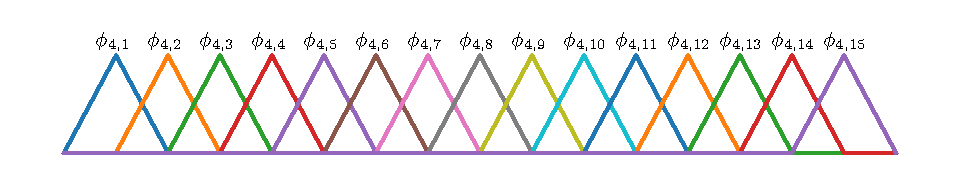
\includegraphics[width=\textwidth]{nodal_basis.pdf}
        \caption{Nodal Basis}
        \label{fig:nodalbasis}
    \end{subfigure}
    \begin{subfigure}{0.45\textwidth}
        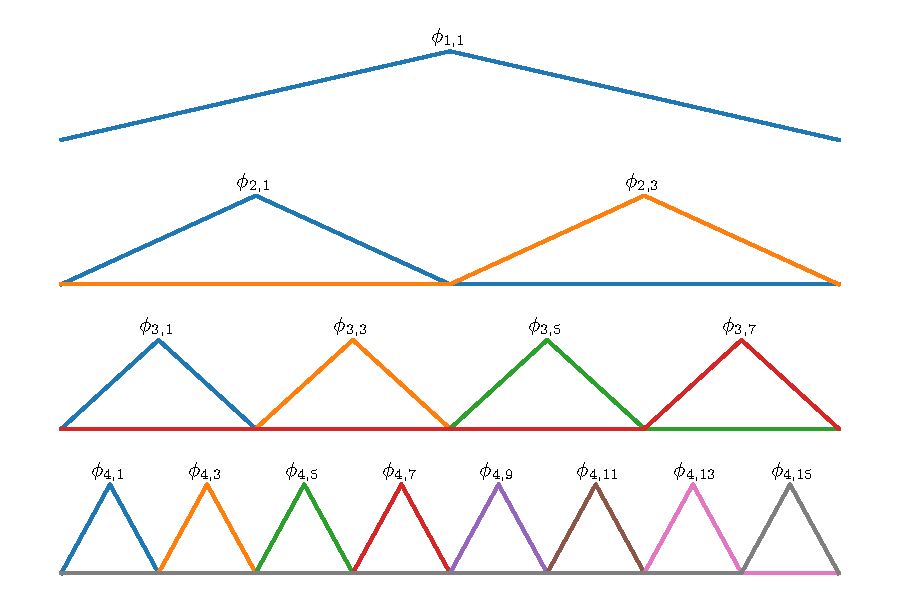
\includegraphics[width=\textwidth]{hierarchical_basis.pdf}
        \caption{Hiearchical Basis}
        \label{fig:hierarchicalbasis}
    \end{subfigure}
    \caption{Comparision of piecewise linear basis functions.}
    \label{fig:basiscomp}
\end{figure}

\begin{table}[hbpt]
    \centering
    \caption{Comparision of Sparse and Full Grid Approaches.}
    \begin{tabular}{l c c}
        \multicolumn{1}{c}{} & Storage Requirement  & \multicolumn{1}{c}{L2 Norm of Interpolation Error} \\
        \toprule
        Full Grid            & \(O(2^{nd})\)        & \(O(2^{-2n})\)                                     \\
        \midrule
        Sparse Grid          & \(O(2^{n} n^{d-1})\) & \(O(2^{-2n} n^{d-1})\)                             \\
        \bottomrule
    \end{tabular}
    \label{tab:comparisionfull}
\end{table}

In this work we will use standard hat function given by \cref{eqn:basis}.

\begin{equation}
    \phi(x ) = \left\{
    \begin{array}{ll}
        1-|x| & \text{if } x \in [-1,1] , \\
        0     & \text{otherwise}          \\
    \end{array}
    \right.
    \label{eqn:basis}
\end{equation}

On a equidistant grid \(\Omega_l \) of level \( l\) on a unit interval \(\bar{\Omega} = [0,1]\). The mesh width is given by \(2^{-l} \). The grid points on a certain level is given bibliography

\begin{equation}
    x_{l,i} = i \cdot h_l, 0 \leq i \leq 2^l
\end{equation}

Using \cref{eqn:basis} a family of basis functions \(\phi_{l,i}(x)\) with a support of \([x_{l,i}-h_l,x_{l,i}+h_l]\), by dilation and translation one could get \cref{eqn:levelbasis}. This process gives all possible basis function in level \(l\) as shown in \cref{fig:nodalbasis}.

\begin{equation}
    \phi_{l,i}(x) = \phi \left(\frac{x-i\cdot h_l}{h_l}\right)
\end{equation}

\begin{equation}
    V_l = \text{span} \left\{ \phi_{l,i} : 1 \leq i \leq 2^l-1 \right\}
    \label{eqn:levelbasis}
\end{equation}

One need hierarchical ones in order to construct the sparse grid. The hierarchical increment spaces are given by \cref{eqn:hierarchicalincrementspace}.

\begin{equation}
    W_l = \text{span} \left\{ \phi_{l,i} : i \in I_l\right\}
    \label{eqn:hierarchicalincrementspace}
\end{equation}

where the index set is,

\begin{equation}
    I_l = \left\{ i \in \mathbb{N}: 1 \leq i \leq 2^l-1 , i \text{ odd} \right\}
\end{equation}

Using the resulting basis functions as input to the tensor product construction, one can obtain suitable piecewise d-linear basis function at each grid point \(x_{l,i}\)

\begin{equation}
    \phi_{l,i}(x) = \prod_{j=1}^d \phi_{l_j,i_j}(x_j)
\end{equation}


\section{Sparse Grids}\label{sec:sparsegrid}

Sparse grids offer a new way to reduce the required number of grid points by order of magnitude \(O(2^{nd})\) to just only \(O(2^n n^{d-1})\) while preserving a similar error as using the full grid~\cite{Garcke2012}.
A comparison of storage requirement and error is listed in \cref{tab:comparisionfull}.
In order to achieve these bounds, the mixed second derivatives must be bounded.

The sparse grid uses a hierarchical formulation as shown in \cref{fig:basiscomp} for a one-dimensional case.
It has an incremental and adaptive behavior inherently. In order to extend to a general d-dimensional setting, it exploits
the tensor product approach.

One can use the advantage of adaptivity for problems that do not satisfy smoothness criteria or require further reduction in mesh size.
The hierarchical basis is a direct indicator of areas where further refinement is required.

\begin{figure}
    \centering
    \begin{subfigure}{0.45\textwidth}
        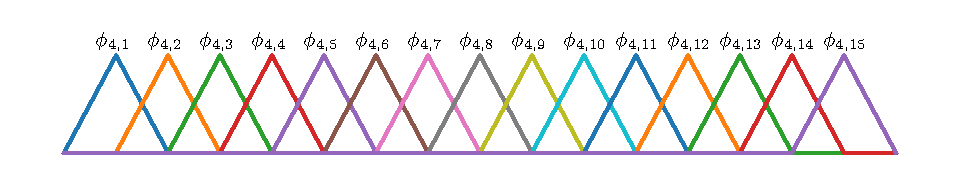
\includegraphics[width=\textwidth]{nodal_basis.pdf}
        \caption{Nodal Basis}
        \label{fig:nodalbasis}
    \end{subfigure}
    \begin{subfigure}{0.45\textwidth}
        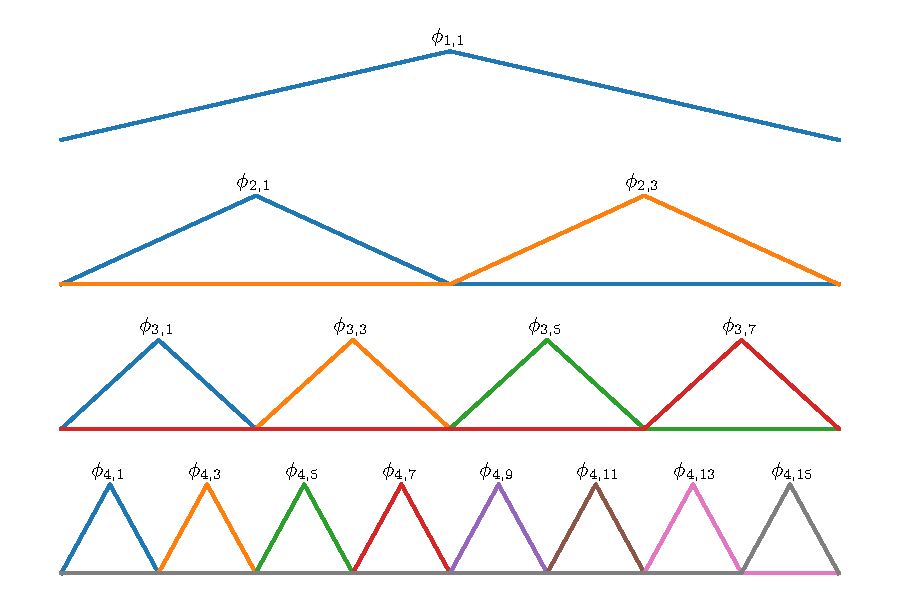
\includegraphics[width=\textwidth]{hierarchical_basis.pdf}
        \caption{Hiearchical Basis}
        \label{fig:hierarchicalbasis}
    \end{subfigure}
    \caption{Comparision of piecewise linear basis functions.}
    \label{fig:basiscomp}
\end{figure}

\begin{table}[hbpt]
    \centering
    \caption{Comparision of Sparse and Full Grid Approaches.}
    \begin{tabular}{l c c}
        \multicolumn{1}{c}{} & Storage Requirement  & \multicolumn{1}{c}{L2 Norm of Interpolation Error} \\
        \toprule
        Full Grid            & \(O(2^{nd})\)        & \(O(2^{-2n})\)                                     \\
        \midrule
        Sparse Grid          & \(O(2^{n} n^{d-1})\) & \(O(2^{-2n} n^{d-1})\)                             \\
        \bottomrule
    \end{tabular}
    \label{tab:comparisionfull}
\end{table}

In this work we will use standard hat function given by \cref{eqn:basis}.

\begin{equation}
    \phi(x ) = \left\{
    \begin{array}{ll}
        1-|x| & \text{if } x \in [-1,1] , \\
        0     & \text{otherwise}          \\
    \end{array}
    \right.
    \label{eqn:basis}
\end{equation}

On a equidistant grid \(\Omega_l \) of level \( l\) on a unit interval \(\bar{\Omega} = [0,1]\). The mesh width \(h_l\) is given by \(2^{-l} \). The grid points on a certain level is given by

\begin{equation}
    x_{l,i} = i \cdot h_l, 0 \leq i \leq 2^l
\end{equation}

Using \cref{eqn:basis} a family of basis functions \(\phi_{l,i}(x)\) with a support of \([x_{l,i}-h_l,x_{l,i}+h_l]\), by dilation and translation one could get \cref{eqn:levelbasis}. This process gives all possible basis function in level \(l\) as shown in \cref{fig:nodalbasis}.

\begin{equation}
    \phi_{l,i}(x) = \phi \left(\frac{x-i\cdot h_l}{h_l}\right)
\end{equation}

\begin{equation}
    V_l = \text{span} \left\{ \phi_{l,i} : 1 \leq i \leq 2^l-1 \right\}
    \label{eqn:levelbasis}
\end{equation}

One needs hierarchical ones in order to construct the sparse grid. The hierarchical increment spaces are given by \cref{eqn:hierarchicalincrementspace}.

\begin{equation}
    W_l = \text{span} \left\{ \phi_{l,i} : i \in I_l\right\}
    \label{eqn:hierarchicalincrementspace}
\end{equation}

where the index set is,

\begin{equation}
    I_l = \left\{ i \in \mathbb{N}: 1 \leq i \leq 2^l-1 , i \text{ odd} \right\}
\end{equation}

Using the resulting basis functions as input to the tensor product construction, one can obtain a suitable piecewise d-linear basis function at each grid point \(x_{l,i}\)

\begin{equation}
    \phi_{l,i}(x) = \prod_{j=1}^d \phi_{l_j,i_j}(x_j)
\end{equation}

More information can be found on Bungartz~\cite{Bungartz2004}.

\section{Adaptivity}

A regular sparse grid is constructed in a way that takes a cut in diagonal hyperplane, which means
it treats all the dimensions equally. However, there can be an importance difference between the dimensions,
i.e. one dimension might be more important than others. This can be solved by so called dimensional adaptivity.

The most straightforward approach for this type of refinement is adding some
new subspaces in the dimension which function changes rapidly. In order to add a new subspace
\(W_{\vec{l}}\) one should include all the backward neighbours in the current set of subspaces.
This refiment treads all the grid points in one dimension as a uniform way,and called as
dimensionally adaptive refinement. Leads more point in one dimension than other one.

\todok{May be add an example of dimensionally adaptive sparse grid to here.}

Morever, there are some cases exist, where dimensional adaptivity is not to be enough to solve problem.
For instance take a function that is mostly flat, have peaks at certain regions in the domain.
Franke's function is a good example for this~\cite{Franke1979}.

\begin{equation}
    \begin{aligned}
        f(\textbf{x}) & = \frac{3}{4} \exp \left( - \frac{(9x_1-2)^2}{4} - \frac{(9x_2-2)^2}{4} \right) \\
                      & + \frac{3}{4} \exp  \left( - \frac{(9x_1+1)}{49} - \frac{9x_2+1}{10}\right)     \\
                      & + \frac{1}{2} \exp \left( -\frac{(9x_1-7)^2}{4} - \frac{(9x_2-3)^2}{4} \right)  \\
                      & - \frac{1}{5} \exp \left( - (9x_1-4 )^2 -(9x_2-7)\right)
    \end{aligned}
\end{equation}

\begin{figure}
    \centering
    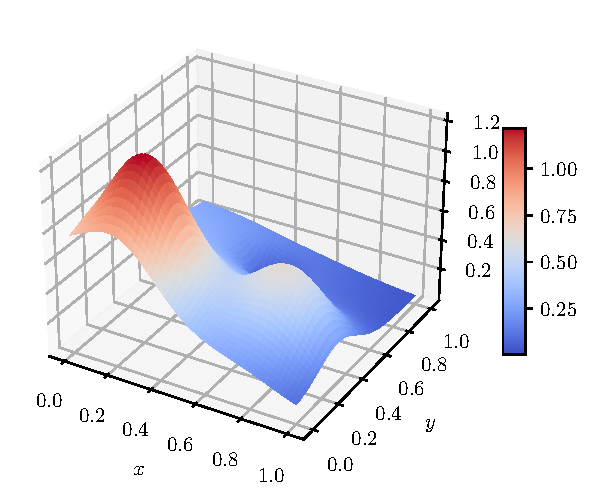
\includegraphics[width=0.4\textwidth]{figures/franke.pdf}
    \caption{Surface plot of Franke's Function.}
    \label{fig:franke}
\end{figure}

A dimensionally adaptive grid would also add more point to regions where the function is mostly flat.
A spatially adaptive grid would overcome this problem. Instead of adding whole incremental grids,
spatial adaption would only include a subset of those points near the region of interest and saves points.

The general approach for spatially adaptive grids is doing the refinement process iteratively.
One could start and initial coarse grid or if knows a grid which is tailored to problem. Using an iterative process
one could simply adds new points (neighboring grid point in the next higher level) to region of interest. To enable usage
of sparse grids algorithms there is also a consistency constraint exist, the grid should contain all the hierarchical
ancestors of all grid points. Figure~\ref{fig:spatialrefiment} shows how this process is done in two-dimensional regular sparse grid.

\begin{figure}
    \centering
    \missingfigure{Add refiment figure here.}
    \caption{Spatial refinement of a selected node in two dimension.}
    \label{fig:spatialrefiment}
\end{figure}


\section{Examples}


\subsection{Spatial Adaptivity}




\section{Conclusion}\label{sec:conclusion}

In this work, we have shown examples of spatially adaptive sparse grid method for multidimensional interpolation problems that can be used to solve a wide range of problems.
The main idea is to use a sparse grid to construct a multidimensional basis of functions that can be used to interpolate a function on a given domain and use an adaptive refinement scheme to adapt the grid to the function's
local behavior.

For demonstrative purposes, we have used free and open-source software SG\textsuperscript{++} to construct the sparse grids and adaptation.
We have used a surplus-based adaptation strategy to adapt the grid to the function's local behavior.

It has already known that a sparse grid method is a powerful tool for solving multidimensional problems without suffering from the curse of dimensionality.
It has also been shown that the sparse grid method can be extended by employing the spatial adaptation technique to solve problems efficiently with a wide range of local behavior.
The strong and weak points of the method are presented in section~\ref{sec:example}. The smoothness of the function affects the interpolated function on the grid drastically. It has shown that discontinuities can be handled using adaptivity. However, higher cross derivatives are not handled well.
The presented technique can be employed for not only interpolation but also quadrature, regression, classification, and other problems. This enables the use of sparse grids for a wide range of applications.


%%%%%%%%%%%%%%%%%%%%%%%%%%%%%%%%%%%%%%%%%%%%%%%%%%%%%%%%%%%%%%%%%%%%%%%%%%
% 	Acknowledgements
%%%%%%%%%%%%%%%%%%%%%%%%%%%%%%%%%%%%%%%%%%%%%%%%%%%%%%%%%%%%%%%%%%%%%%%%%%

%\section*{Acknowledgment}
%\addcontentsline{toc}{section}{Acknowledgment}

%%%%%%%%%%%%%%%%%%%%%%%%%%%%%%%%%%%%%%%%%%%%%%%%%%%%%%%%%%%%%%%%%%%%%%%%%%
% 	References
%%%%%%%%%%%%%%%%%%%%%%%%%%%%%%%%%%%%%%%%%%%%%%%%%%%%%%%%%%%%%%%%%%%%%%%%%%

% trigger a \newpage just before the given reference
% number - used to balance the columns on the last page
% adjust value as needed - may need to be readjusted if
% the document is modified later
%\IEEEtriggeratref{8}
% The "triggered" command can be changed if desired:
%\IEEEtriggercmd{\enlargethispage{-5in}}

% references section
% NOTE: BibTeX documentation can be easily obtained at:
% http://www.ctan.org/tex-archive/biblio/bibtex/contrib/doc/

% can use a bibliography generated by BibTeX as a .bbl file
% standard IEEE bibliography style from:
% http://www.ctan.org/tex-archive/macros/latex/contrib/supported/IEEEtran/bibtex
\bibliographystyle{IEEEtran}
% argument is your BibTeX string definitions and bibliography database(s)
\bibliography{references,IEEEabrv}
%
% <OR> manually copy in the resultant .bbl file
% set second argument of \begin to the number of references
% (used to reserve space for the reference number labels box)
%\begin{thebibliography}{1}
%
%\bibitem{ref:kopka}
%H.~Kopka and P.~W. Daly, \emph{A Guide to {\LaTeX}}, 3rd~ed.\hskip 1em plus
%  0.5em minus 0.4em\relax Harlow, England: Addison-Wesley, 1999.
%
%\end{thebibliography}

%%%%%%%%%%%%%%%%%%%%%%%%%%%%%%%%%%%%%%%%%%%%%%%%%%%%%%%%%%%%%%%%%%%%%%%%%%
% 	End of the document
%%%%%%%%%%%%%%%%%%%%%%%%%%%%%%%%%%%%%%%%%%%%%%%%%%%%%%%%%%%%%%%%%%%%%%%%%%

\end{document}

